\subsection{Обзор литературы}

\subsubsection{Общие сведения о диффузионных моделях}
\par
Долго лидирующие на поприще генерации изображений генеративно-состязательные сети обладают набором проблем, с которыми боролось и продолжает бороться научное сообщество. Основными проблемами, сохранившимися до сих пор, являются нестабильность обучения \cite{kodali2017convergence}, решаемая с помощью спектральной нормализации \cite{miyato2018spectral}, контролирующей константу Липшица, вводя ограничение весов, для стабилизации обучения дискриминатора; Mode Collapse \cite{thanhtung2020catastrophic}. Последняя является одной из главных проблем моделей такого типа. Проблема заключается в том, что в процессе обучения генератор приходит к состоянию, при котором генерируется лишь ограченный (существенно меньший оригинального пространства изображений) набор выходов. Предлагаемые решения этой проблемы -- WGAN \cite{arjovsky2017wasserstein} (авторы используют метрику Вассерштейна внутри лосс-функции, тем самым мотивируя дискриминатор выявлять повторяющие выходы, в которых стабилизировался генератор) и UGAN \cite{metz2017unrolled} (также адаптация функции потерь, однако теперь с оценкой выходов генератора на основе предсказаний будущих версий дискриминатора).

\par
В отличие от генеративно-состязательных сетей эти же проблемы не свойственны новому классу моделей -- диффузионным моделям. В оригинальной статье \cite{sohldickstein2015deep} авторы утилизируют идею из статистической термодинамики. Главной целью авторы видят определение двух процессов: итеративный диффузный процесс, который преобразует любое комплекное распределение данных в более простое и контролируемое, постепенно уменьшая SNR (signal-to-noise ratio), а также параметризованный обратный диффузионный процесс, обучаемый итеративно моделировать целевое распределение.


\textbf{Прямой процесс}

\par
Рассмотрим набор данных из сложно контролируемого целевого распределения: $X = (x^1, \ldots, x^n)$. Построим прямой процесс диффузии, постепенно зашумляющий данные из целевого распределения (уменьшая SNR).
\[
    \begin{array}{c}
        x^i_0 \to x^i_1 \to \ldots \to x^i_T\\
        x^i_{t} = \sqrt{1-\beta_t}\cdot x^i_{t-1} + \sqrt{\beta_t}\cdot \epsilon, \hspace*{0.5cm} \epsilon \sim \mathcal{N}(\epsilon| \ 0, \ I)
    \end{array}
\]
где $\beta_t$ -- скорость диффузии на шаге $t$, $x^i$ -- семпл из выборки (сейчас и далее просто $x$). Этот прямой диффузионный процесс может быть записан в следующем виде:
\begin{equation}
    q(x_{t}|x_{t-1}) = \mathcal{N}(x_{t} \vert \sqrt{1 - \beta_t}x_{t-1}, \beta_t I)
    \label{eq:forward_process}
\end{equation}
\begin{figure}[H]
    \centering
    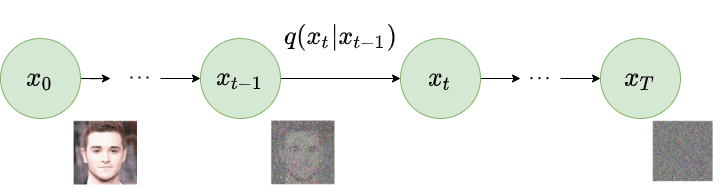
\includegraphics[scale=0.5]{forward-diffusion.png}
    \caption{Прямой процесс диффузии \cite{ho2020denoising}}
    \label{fig:forward_process}
\end{figure}
Используя трюк с репараметризаций можно получить явное выражение для семплирования на каждом шаге диффузии (\hyperref[AppendixA]{ПРИЛОЖЕНИЕ 1}):
\begin{equation}
    x_t \sim q(x_t| x_0) = \mathcal{N}(x_t\vert \sqrt{\overline{\alpha}_t} x_0, \ (1 - \overline{\alpha}_t)I),    
    \label{eq:any_step}
\end{equation}
где $\overline{\alpha_t} = \prod_{s=0}^{t} (1 - \beta_t)$. Из последнего выражения нетрудно заметить, что при $T \to \infty \Longrightarrow \overline{\alpha}_T \to 0$  генерируемый семпл будет иметь стандартное нормальное распределение $x_T \sim \mathcal{N}(x^T\vert 0, I)$. 

\textbf{Обратный процесс}

Построив обратный процесс: $q(x_{t-1}\vert x_t)$ будет возможно воссоздать истинную выборку по входному сигналу гауссова шума. В условиях выбора малых $\beta_t$ можно гарантировать, что $q(x_{t-1}| x_t)$ также гауссово распределение. Однако, оценка $q(x_{t-1}\vert x_t)$ невозможна без генеральной совокупности. В статье \cite{sohldickstein2015deep} предлагается параметризовать оценку условной вероятности $p_\theta$ для запуска процесса обратной диффузии: 
\begin{equation}
    p_\theta(x_{t-1}\vert x_t) = \mathcal{N}(x_{t-1}\vert \mu_\theta(x_t, t), \Sigma_\theta(x_t, t))    
\end{equation}
\begin{figure}[H]
    \centering
    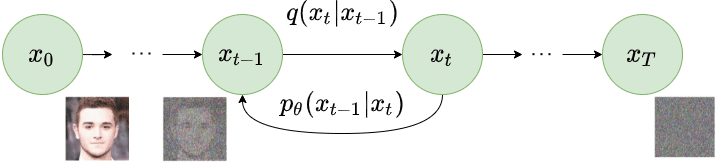
\includegraphics[scale=0.5]{reverse-diffusion.png}
    \caption{Обратный процесс диффузии \cite{ho2020denoising}}
    \label{fig:reverse_process}
\end{figure}

% не до конца понял
Обратная условная вероятность $q(x_{t-1}\vert x_t)$ контролируема, если обусловлена на $x_0$:
\begin{equation}
    q(x_{t-1}\vert x_t, x_0) = \mathcal{N}(x_{t-1}, \tilde{\mu}(x_t, x_0), \tilde{\beta}_t  I)  
    \label{eq:controlable_condition}
\end{equation}
причем из \ref{eq:any_step} следует можно выразить:
\[
    \begin{array}{c}
        \tilde{\beta}_t = \dfrac{1 - \overline{\alpha}_{t-1}}{1 - \overline{\alpha}_t} \cdot \beta_t,  \\[0.5cm]
        \tilde{\mu}_t(x_t, x_0) = \dfrac{}{} x_0 + \dfrac{\sqrt{\alpha_t}(1 - \overline{\alpha}_{t-1})}{1-\overline{\alpha}_t} x_t
    \end{array}
\]
Пользуясь результатами \hyperref[AppendixA]{ПРИЛОЖЕНИЕ 1.} можно выразить:
\[
    x_0 = \dfrac{1}{\sqrt{\overline{\alpha}_t}} (x_t - \sqrt{1 - \overline{\alpha}_t \epsilon})  
\]
Собирая вместе два последних выражения, можем получить среднее для произвольного шага, зависящее от $x_t$:
\[
    \tilde{\mu}_t(x_t) = \dfrac{1}{\sqrt{\alpha_t}} \left(x_t - \dfrac{\beta_t}{\sqrt{1 - \overline{\alpha}_t}}\epsilon\right)
\]
В статье \cite{ho2020denoising} предлагается использовать нейронную сеть для оценки шума:
\[
    \tilde{\mu}_\theta(x_t, t) = \dfrac{1}{\sqrt{\alpha_t}}\left(x_t - \dfrac{\beta_t}{\sqrt{1 - \overline{\alpha}_t}}\epsilon_\theta(x_t, t)\right)  
\]
Тогда функция ошибки (подробнее в \hyperref[AppendixC]{ПРИЛОЖЕНИЕ 3.}) может быть выражена:
\[
    L_t = \mathbb{E}_{x_0, t, \epsilon}\left[\dfrac{1}{2||\Sigma_\theta(x_t, t)||_2^2} ||\tilde{\mu}_t - \tilde{\mu}_\theta(x_t, t)||_2^2\right] = \mathbb{}_{} \left[\dfrac{1}{2||\Sigma_\theta(x_t, t)||_2^2} ||\epsilon_t - \epsilon_\theta(\sqrt{\overline{\alpha}_t}x_0 + \sqrt{1 - \overline{\alpha}_t}\epsilon, t)||^2\right]
\]
В статье \cite{ho2020denoising} авторы обнаружили, что обучение модели лучше работает с упрощенным лоссом, с опущенным весовым членом
\[
    L_t^* = \mathbb{E}_{x_0, t, \epsilon}\left[||\epsilon_t - \epsilon_\theta(\sqrt{\overline{\alpha}_t}x_0 + \sqrt{1 - \overline{\alpha}_t}\epsilon, t)||^2\right]  
\]
Но в \cite{nichol2021improved} авторы показывают, что если учить оценку ковариационной матрицы, то результат будет лучше.
\begin{figure}[H]
    \centering
    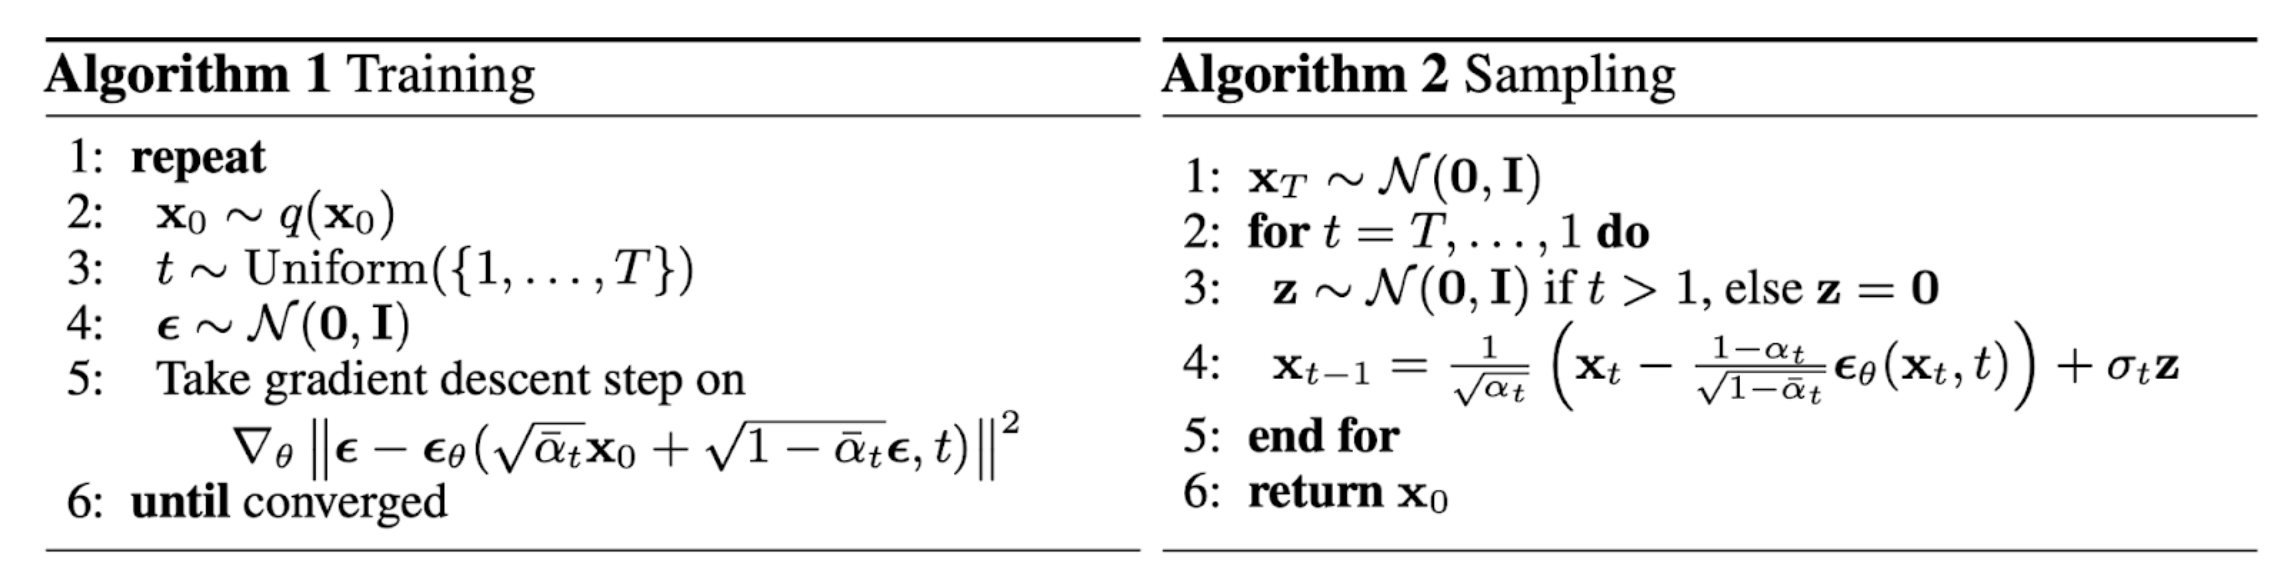
\includegraphics[scale=0.4]{DDPM-algo.png}
    \caption{Алгоритмы обучения и семплирования \cite{ho2020denoising}}
    \label{fig:algo_ddpm}
\end{figure}

% TODO: sheduling \beta_t
% TODO: архитектура


% не до конца понял
% \par
% Динамика Ланжевена \cite{10.5555/3104482.3104568} позволяет сэмплировать из плотности распределения используя только градиенты $\dfrac{\partial}{\partial x} \log p(x)$



% Процедура \ref{eq:Langevene} представляет собой градиентный подъем, который направлен на нахождение моды распределения, однако, что является большим преимуществом перед генеративно-состязательными сетями: происходит зашумление градиента, что релаксирует высокие значения плотности распределения. 

\par

% ! дописать


\subsubsection{Обуславливаемые диффузионные модели (Conditioned diffusion models)}
\par

В статье \cite{rombach2022highresolution} предлагается модель латентной диффузии. Авторы представляют процесс диффузии не в пространстве пикселей, а в пространстве латентных эмбеддингов, полученных с помощью автоэнкодера (VQ-VAE). Авторы обнаружили, что даже агрессивная компрессия сохраняет семантическую и концептуальную информацию \ref{fig:image-distortion-rate}. Поэтому они сначала убирают избыточность (компрессируют) с помощью автоэнкодера, а затем манипулируют/генерируют семантические понятия с помощью процесса диффузии на выученном латентном уровне. Энкодер $\mathcal{E}$ используется для компрессии входных изображений в латентные эмбеддинги: $z = \mathcal{E}(x^{H\times W\times 3}) \in \mathbb{R}^{h\times w\times c}$. Затем для реконструкции из латентного пространства используется декодер $\mathcal{D}:\ \hat{x} = \mathcal{D}(z)$.
\begin{figure}[H]
    \centering
    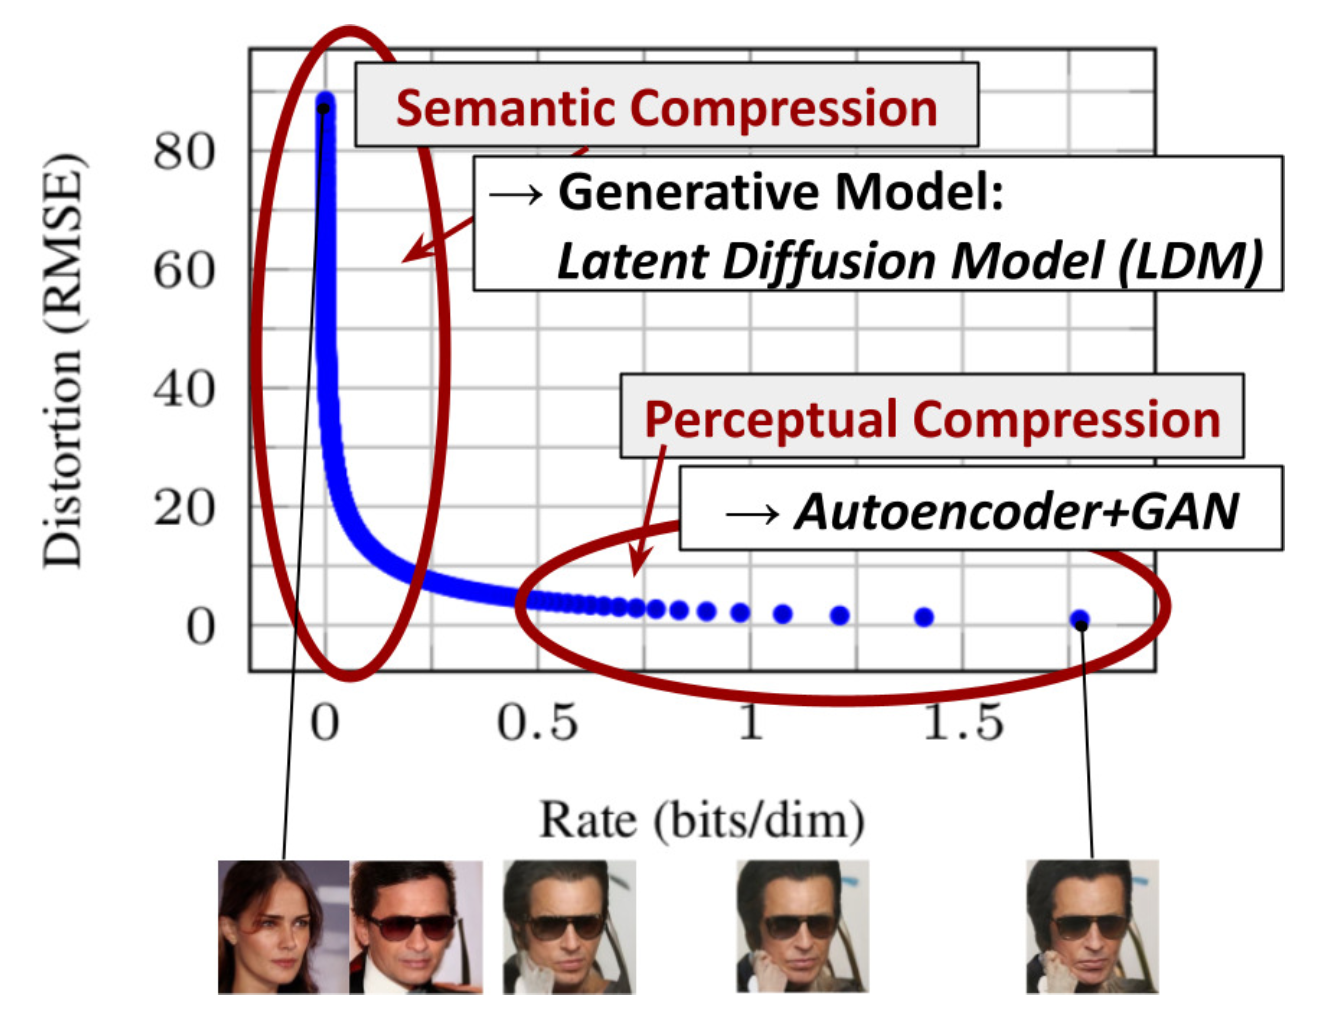
\includegraphics[scale=0.4]{image-distortion-rate.png}
    \caption{Trade-off между сжатием и соответствующими искажениями \cite{rombach2022highresolution}}
    \label{fig:image-distortion-rate}
\end{figure} 

В статье предлагается два типа регуляризации в обучении автоэнкодера чтобы избежать высокой дисперсии в латентном пространстве:
\begin{itemize}
    \item $KL$-регуляризация, взятая из идеи VAE \cite{Kingma_2019}, штраф за $KL$ дивергенцию между распределением в латентном пространстве и стандартным нормальном распределением.
    \item $VQ$-регуляризация, взятая из идеи VQVAE \cite{oord2018neural}, использующая векторную квантизацию внутри декодера.
\end{itemize}

\par
Прямой и обратный процессы диффузии происходят в латентном представлении $z$. Архитектурой была выбрана $U-Net$, обусловленная по шагу диффузии с добавлением механизма перекрестного внимания, который позволяет обуславливать генерацию под разный тип данных (метки классов, low-pass изображения, текстовые запросы). 
\[
    \begin{aligned}
    &\text{Attention}(Q, K, V) = \text{softmax}\Big(\frac{QK^\top}{\sqrt{d}}\Big) \cdot V \\
    &\text{where }Q = W^{(i)}_Q \cdot \varphi_i(z_i),\;
    K = W^{(i)}_K \cdot \tau_\theta(y),\;
    V = W^{(i)}_V \cdot \tau_\theta(y) \\
    &\text{and }
    W^{(i)}_Q \in \mathbb{R}^{d \times d^i_\epsilon},\;
    W^{(i)}_K, W^{(i)}_V \in \mathbb{R}^{d \times d_\tau},\;
    \varphi_i(z_i) \in \mathbb{R}^{N \times d^i_\epsilon},\;
    \tau_\theta(y) \in \mathbb{R}^{M \times d_\tau}
    \end{aligned}
\]

\begin{figure}[H]
    \centering
    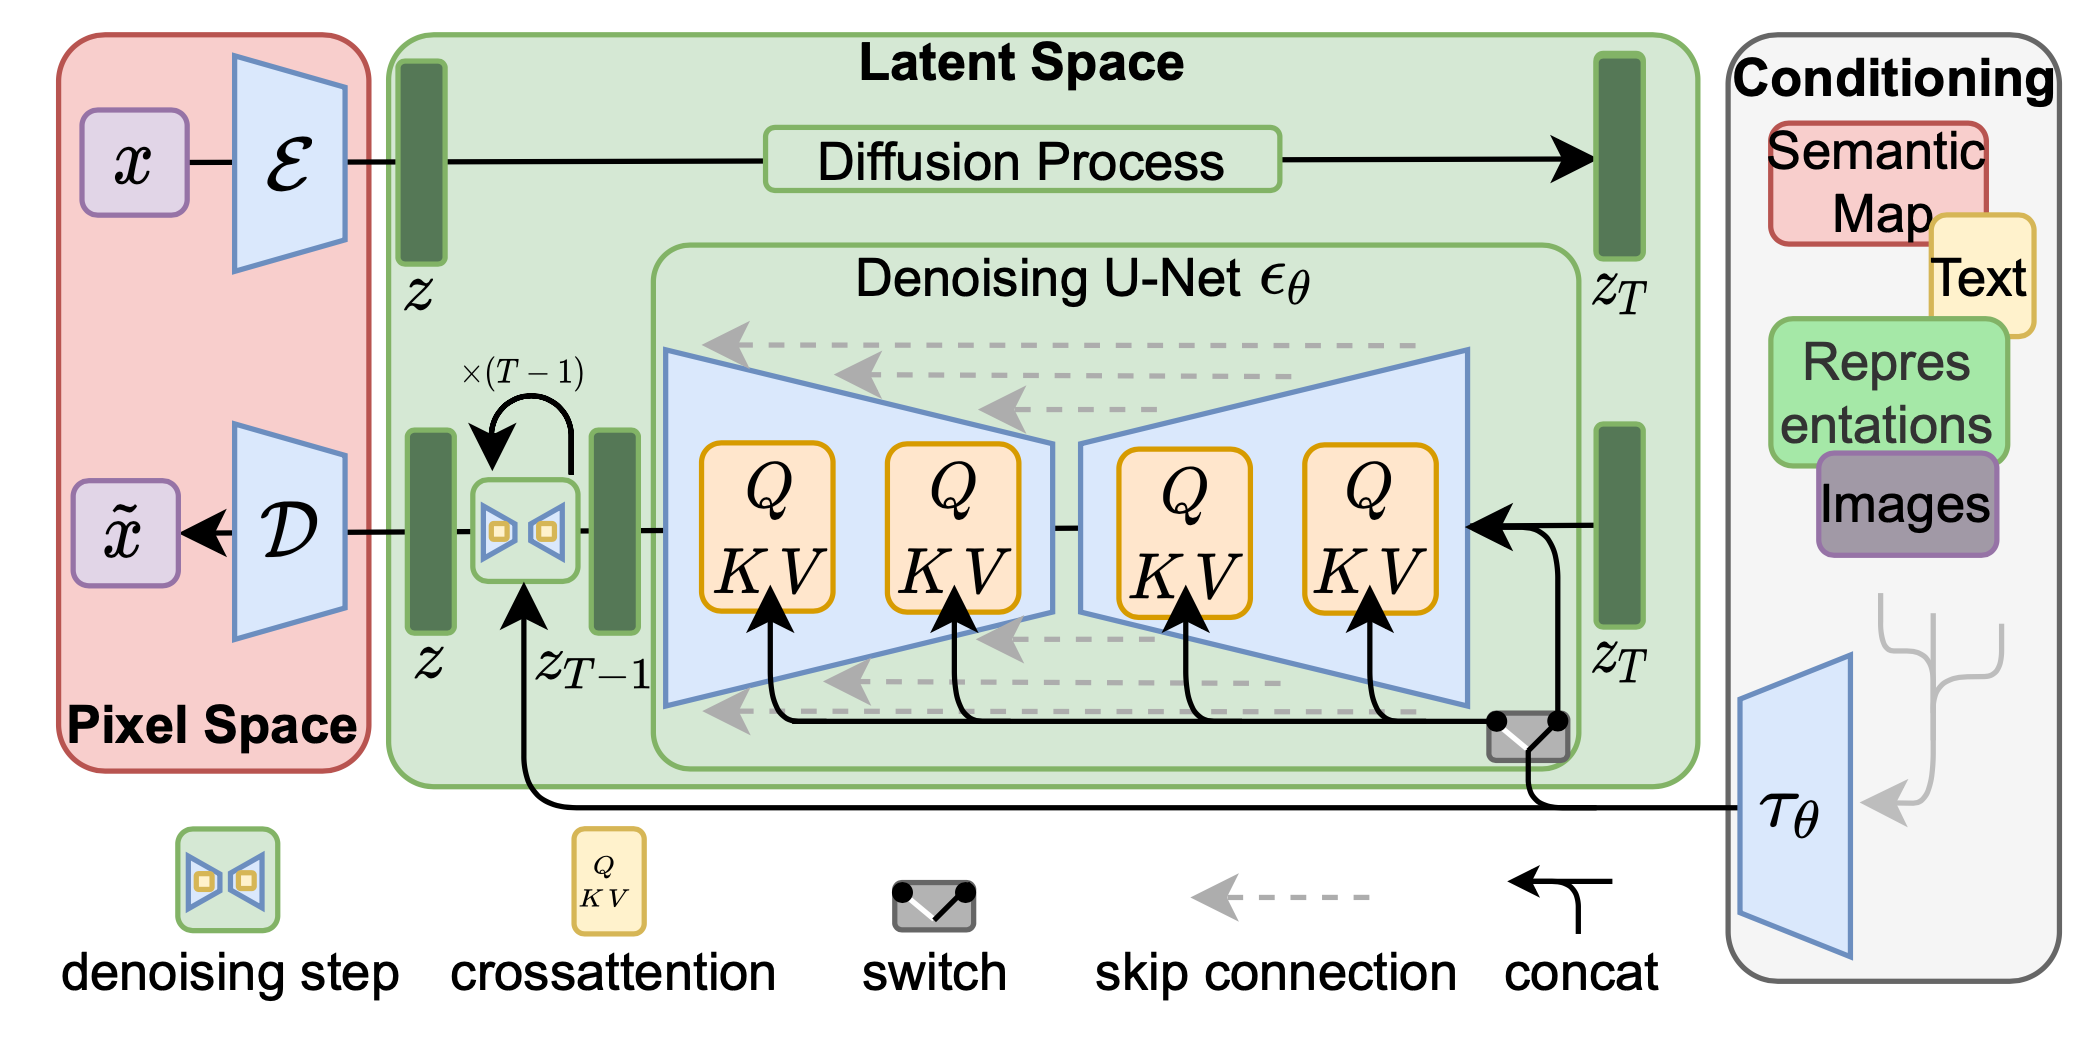
\includegraphics[scale=0.4]{latent-diffusion-arch.png}
    \caption{U-Net архитектура с перекрестным вниманием}
    \label{fig:latent-diffusion-arch}
\end{figure} 
% ! дописать
В \cite{ruiz2023dreambooth} предлагается использование концептов. 




\subsubsection{Обучение моделей}
\par

\subsubsection{Задача замены лиц (Face swap)}

\par
В статье \cite{li2020faceshifter} авторы предлагают двухступенчатую архитектуру для решения поставленной задачи. Авторы утилизируют идею генеративно-состязательных сетей, на первом этапе генерирует изображение с помощью адаптивного внедрения признаков из целевого изображения. Генератор в модели основывается на AAD (Adaptive Attentional Denormalization) слоях. На втором этапе модель решает проблему появления артифактов и нереалистичных частей на изображении в self-supervised режиме.  

\begin{itemize}
    \item AEI-Net (Генерация целевого лица):
    
    AEI-Net состоит из энкодера личности (Identity Encoder), многоуровневого энкодера атрибутов (Multi-level Attributes Encoder) и генератора (AAD-Generator). AAD-Generator интегрирует информацию о личности и атрибутах на нескольких уровнях с помощью блоков AAD ResBlks. Такие блоки основываются на AAD слоях.
    \begin{figure}[H]
        \centering
        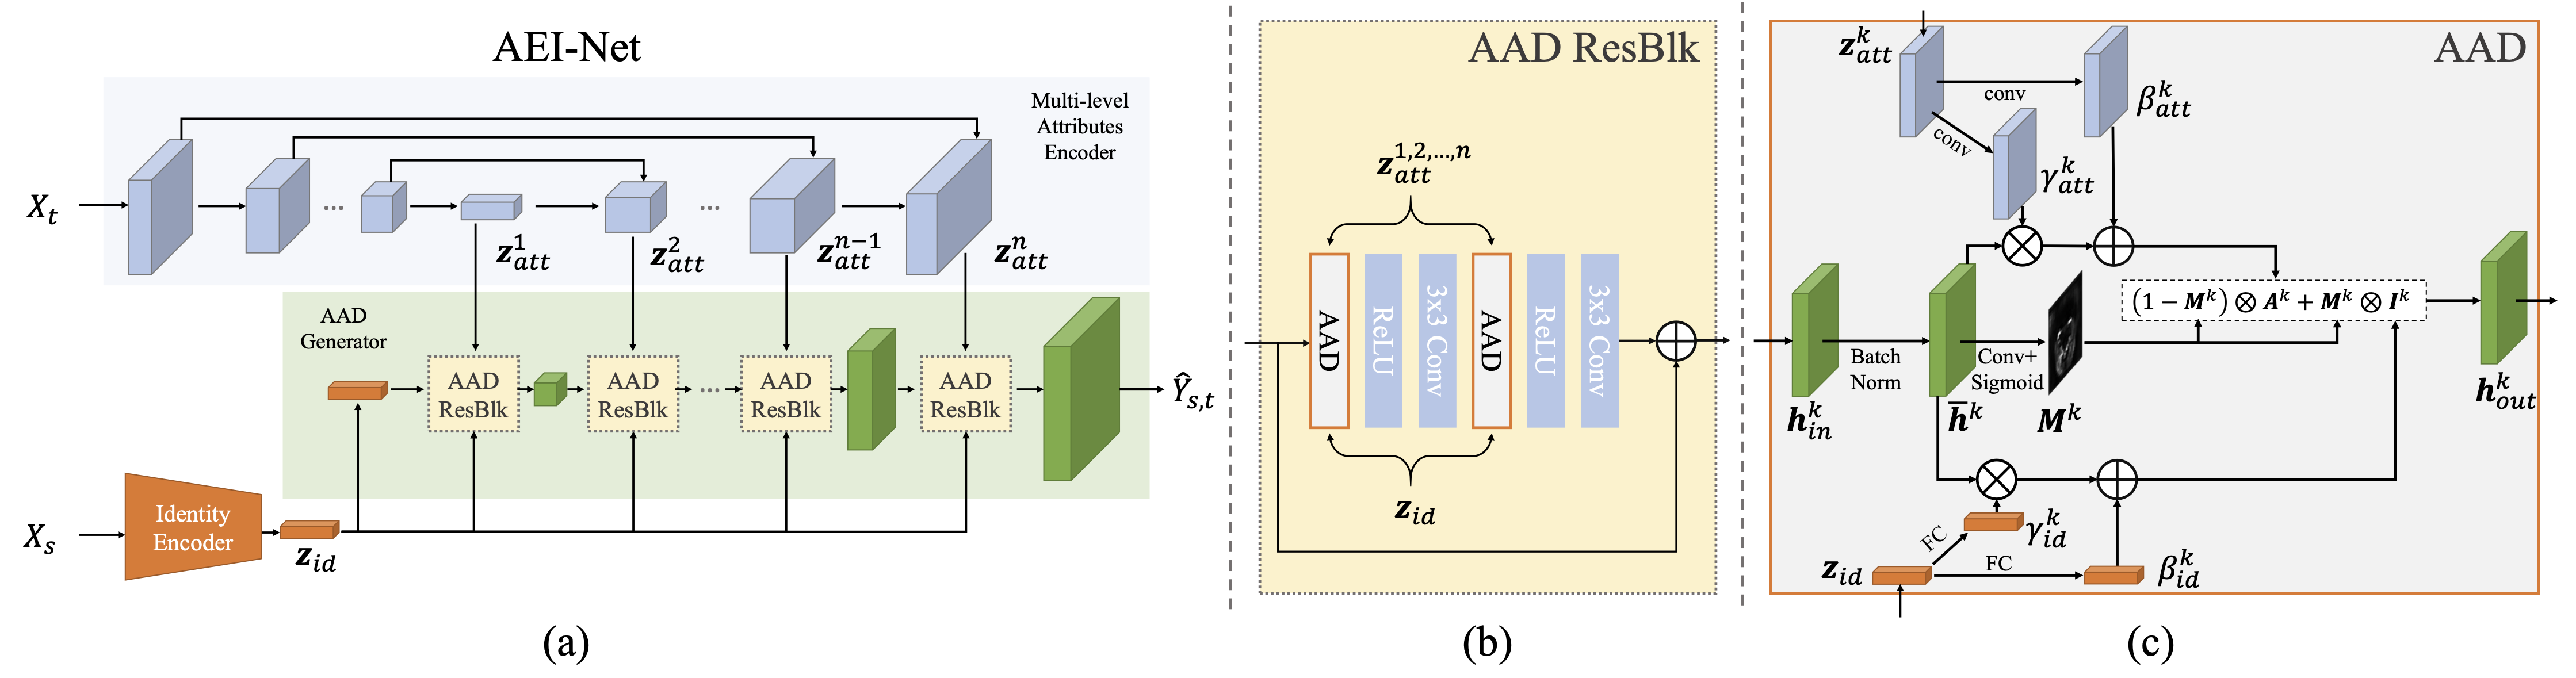
\includegraphics[scale=0.2]{first_step_faceshifter.png}
        \caption{Первый этап FaceShifter \cite{li2020faceshifter}}
        \label{fig:first_step_faceshifter}
    \end{figure} 
    \item HEAR-Net (Избавление от возможных артефактов)
    \begin{figure}[H]
        \centering
        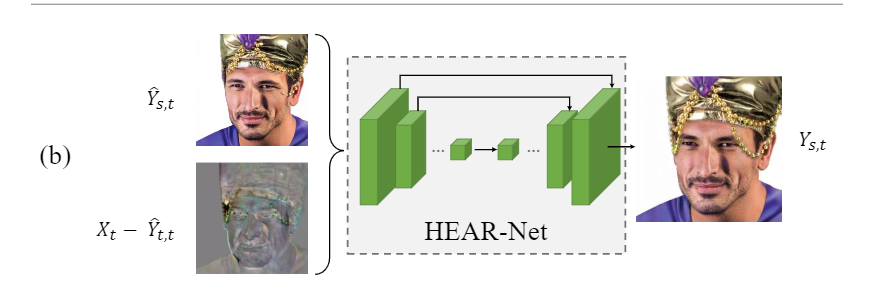
\includegraphics[scale=0.4]{second_step_faceshifter.png}
        \caption{Второй этап FaceShifter \cite{li2020faceshifter}}
        \label{fig:second_step_faceshifter}
    \end{figure}
\end{itemize}
